
\chapter{Presentation of the project}

\section{Context}

During my second year school at ENSTA Bretagne, Mr Champeau taught us UML Diagrams. During this lesson, He shown us the possibility to create Codes from UML Diagram and the possibility to simulate UML Diagrams such as an overview of the running. But to do that, He needed a tool to create UML Model and simulate them. There is only two tools which permit that: Rhapsody and Papyrus.

Papyrus use Moka to simulate UML Model and it was not well adapted for his lesson, so he choose Rhapsody. However, problems are that Rhapsody is not an open source software, it is only for Windows OS, and it is not free. That is why many student said that you won't use this software outside the lesson.

Mr Champeau has proposed this internship to fill in the lack of simulator in open source UML Modelers.

  \begin{figure}[h]
    \begin{minipage}{0.45\linewidth}
      \centering
      
\includegraphics[width=0.7\textwidth]{Rapsody}
      \caption{Rational Rhapsody}
      \label{fig:rhapsody}
    \end{minipage}\hfill
    \begin{minipage}{0.45\linewidth}
      \centering
      
\includegraphics[width=\textwidth]{Papyrus}
      \caption{Papyrus}
      \label{fig:papyrus}
    \end{minipage}
  \end{figure}



\section{The goal}

The goal of this project is to visualize a simulation of Statechart in UML Designer. The simulator should permit to visualize and debug a model of a state machine. Moreover, UML Designer is a modeling software for UML model and Statechart, so we could create the model and simulate it on the same tools. The picture \ref{fig:project} represent the aim of this project.

\begin{figure}[h]
  \centering
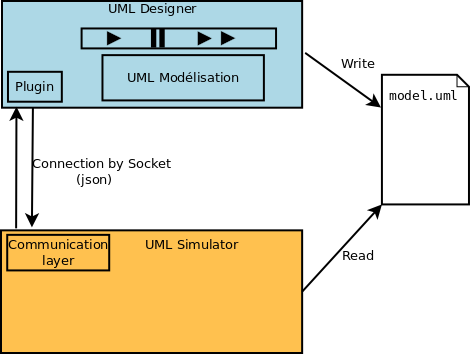
\includegraphics[width=\textwidth]{project}
  \caption{Description of the project}
  \label{fig:project}
\end{figure}


\section{Tools at the disposal}

At the begin of this project, some of the tools, which were needed, existed. In fact, ULMDesigner is a UML modeling tool develop by \textit{Obeo}. However, it didn't exist yet a simulator for Statechart adapted for UMLDesigner. On the chapter \ref{chap:UMLDesigner}, the running of UMLDesigner will be discuss.~\\

Then, Mr Ciprian Theodorov, one of my professor, has developed a simulator for Statechart. This simulator needed to be improved, but it composed a good beginning for this project.



%%% Local Variables:
%%% mode: latex
%%% TeX-master: "../rapport_de_base"
%%% End:
